\subsection{Polykonische Projektion}
\label{sec:polikonisch}
Die polikonische Projektion ist eine globale Projektion. Hierbei werden auf dem zentralen Meridian unendlich viele Kegel aufgebaut. Dabei entstehen nicht konzentrische Breitenkreise. Die Projektion geht an den Polen auseinander. Die Verzerrung der Fläche nimmt mit der Entfernung vom zentralen Meridian der Karte zu. Die Winkel sind lokal entlang des zentralen Längengrades genau, sonst sind sie verzerrt.\\

\begin{figure}[hbtp]
\centering
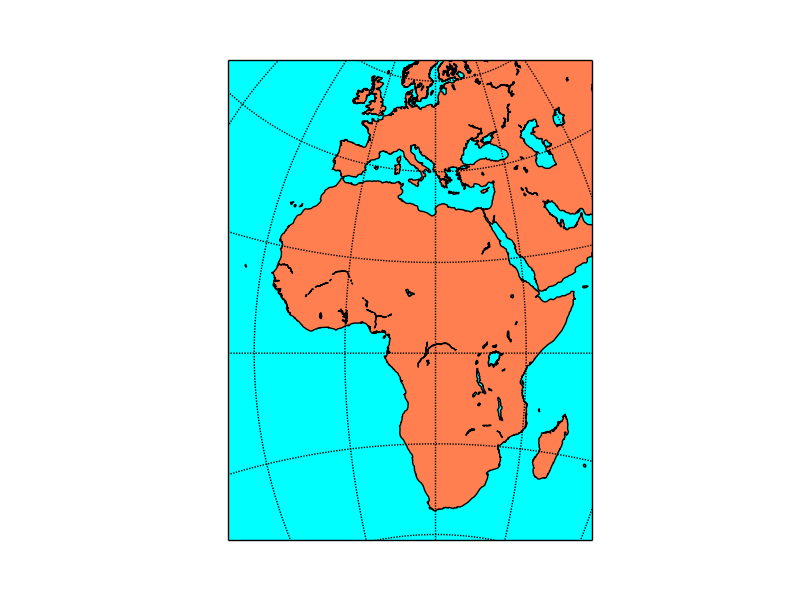
\includegraphics[scale=0.5,origin=c]{/Users/student/seminar/Kartendarstellungen/seminar/poly} \caption{Polykonische Projektion}
\end{figure}
\newpage 